\documentclass[a4paper,11pt]{kth-mag}
\usepackage[T1]{fontenc}
\usepackage{textcomp}
\usepackage{lmodern}
\usepackage[latin1]{inputenc}
\usepackage[swedish,english]{babel}
\usepackage{modifications}

\usepackage{graphicx}
\usepackage{amsmath}
\usepackage{bm}

% Put title here
\title{Weakly Supervised Object Detection: (Working title)}

\subtitle{Duis autem vel eum iruire dolor in hendrerit in
          vulputate velit esse molestie consequat, vel illum
          dolore eu feugiat null}
\foreigntitle{Lorem ipsum dolor sit amet, sed diam nonummy nibh eui
              mod tincidunt ut laoreet dol}
              
\author{Muhammad Iqbal Tawakal}

\date{2015}
\blurb{Master's Thesis at NADA\\Supervisor: Tjoho\\Examiner: Tjohej}
\trita{TRITA xxx yyyy-nn}

\begin{document}
\frontmatter
\pagestyle{empty}
\removepagenumbers
\maketitle
\selectlanguage{english}

\begin{abstract}
  This is a skeleton for KTH theses. More documentation
  regardings the KTH thesis class file can be found in
  the package documentation.
  
  Weakly supervised object detection is...
\end{abstract}

\clearpage
\begin{foreignabstract}{swedish}
  Denna fil ger ett avhandlingsskelett.
  Mer information om \LaTeX-mallen finns i
  dokumentationen till paketet.

\end{foreignabstract}
\clearpage
\tableofcontents*
\mainmatter
\pagestyle{newchap}


\chapter{Introduction}
\label{chap:intro}

% Computer vision history
Computer vision is a field that focused on the process of acquiring, analyzing, and ultimately extracting knowledge and getting comprehensive understanding of the input image. The input image can take many forms such as still image (black and white or colored image), video sequences, multiple input from multiple cameras, and also input from other related sensor. This field has strong ties with other field such as artificial intelligence, machine learning, and robotic.

There are wide range of real world applications for computer vision, starting from simple inspection system in industry and manufacturing process to the creation of robot with artificial intelligence that can interact with  the world around them. Other application include system for navigation (for example autonomous mobile robot and vehicle) and military (security surveillance and missile guidance system).

Those applications can usually be broken down into several small scale vision tasks. Two of the most typical tasks in computer vision are object recognition and object detection. Object recognition tries to predict and identify what class of object is contained inside an image. In detection case, not only the class of the object, the position itself must also be located, usually by marking a tight bounding box closely surrounding the object. Both are hard, challenging problems that are still being actively researched today.

% Reason for difficulty
There are many factors that can be attributed as to why the object recognition and its kind are hard. One reason is simply because the natural representation of image as 2D matrix of pixels value hold little to no direct information that can be used to distinguish different object. Figure \ref{fig:car} illustrate this example. 

This is worsened by the high dimensionality of the data. A standard high definition colored image with the size of 1280x720 can contains up to 2764800 dimensions. Meanwhile the amount of training data rarely exceed or even match this number. This curse of dimensionality can make the training phase to become slow and hard.

\begin{figure}[h]
\centering
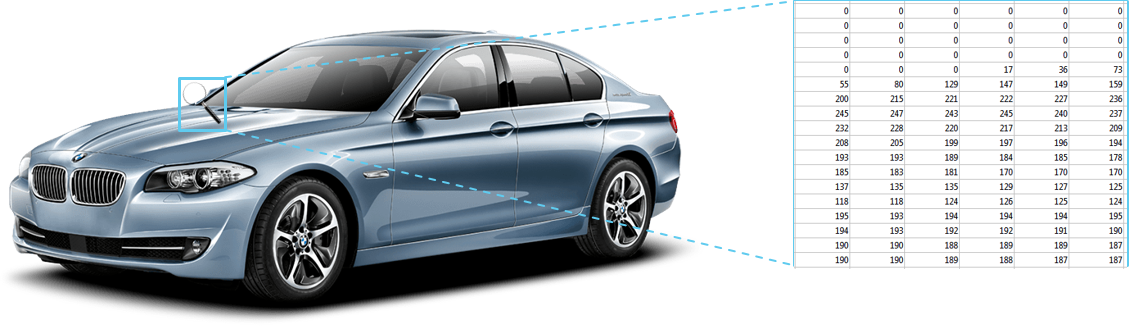
\includegraphics[scale=0.4]{image/car.png}
\label{fig:car}
\caption{The image as 2D matrix of pixels.}
\end{figure}

Furthermore, there are many variations which makes same identical object to have very different appearances in the image. This can be due to viewing changes (translation, rotation, or scale change), change of illumination, occlusion, and clutter. There are also intrinsic difference of object from the same class. Figure \ref{fig:objects} illustrates this example.

\begin{figure}[h]
\centering
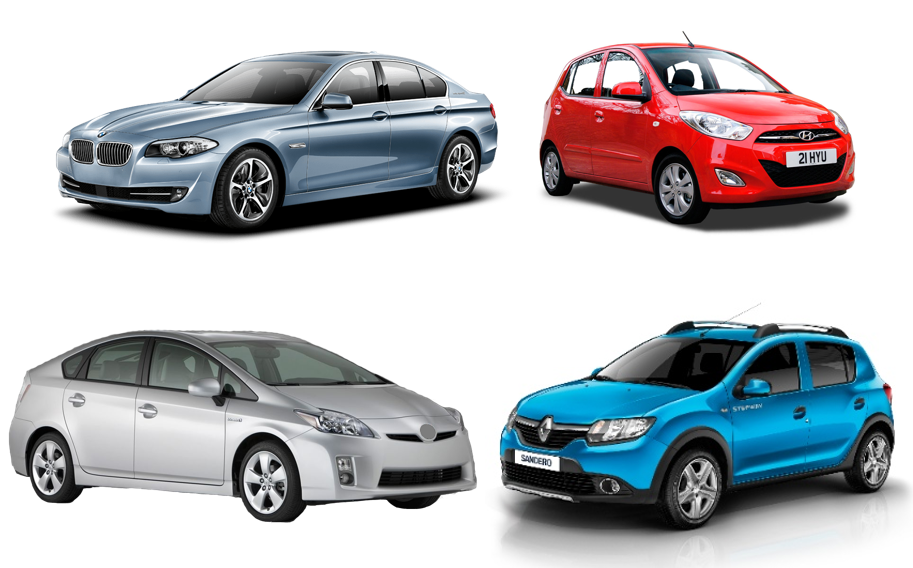
\includegraphics[scale=0.4]{image/cars.png}
\label{fig:cars}
\caption{Object with different appearances, be it color or shape, from the same class.}
\end{figure}

% The importance of features
All this boils down to finding the best representation or features of the said object. An ideal representation would be highly discriminative of different class of object but captures the intrinsic similarity between object from the same class. It also has to be invariant to the object transformation (translation, rotation, and scale invariant), usually have lower number of dimension, and also fast and easy to compute.

Unfortunately, these kind of ideal features do not exist in reality. In practice, we compromise by striking a balance of using adequate number of training data and using a stronger learning algorithm to compensate for the not-so-ideal features. Figure \ref{fig:feature} shows illustration of the ideal features and the not-so-ideal features.

\begin{figure}[h]
\centering
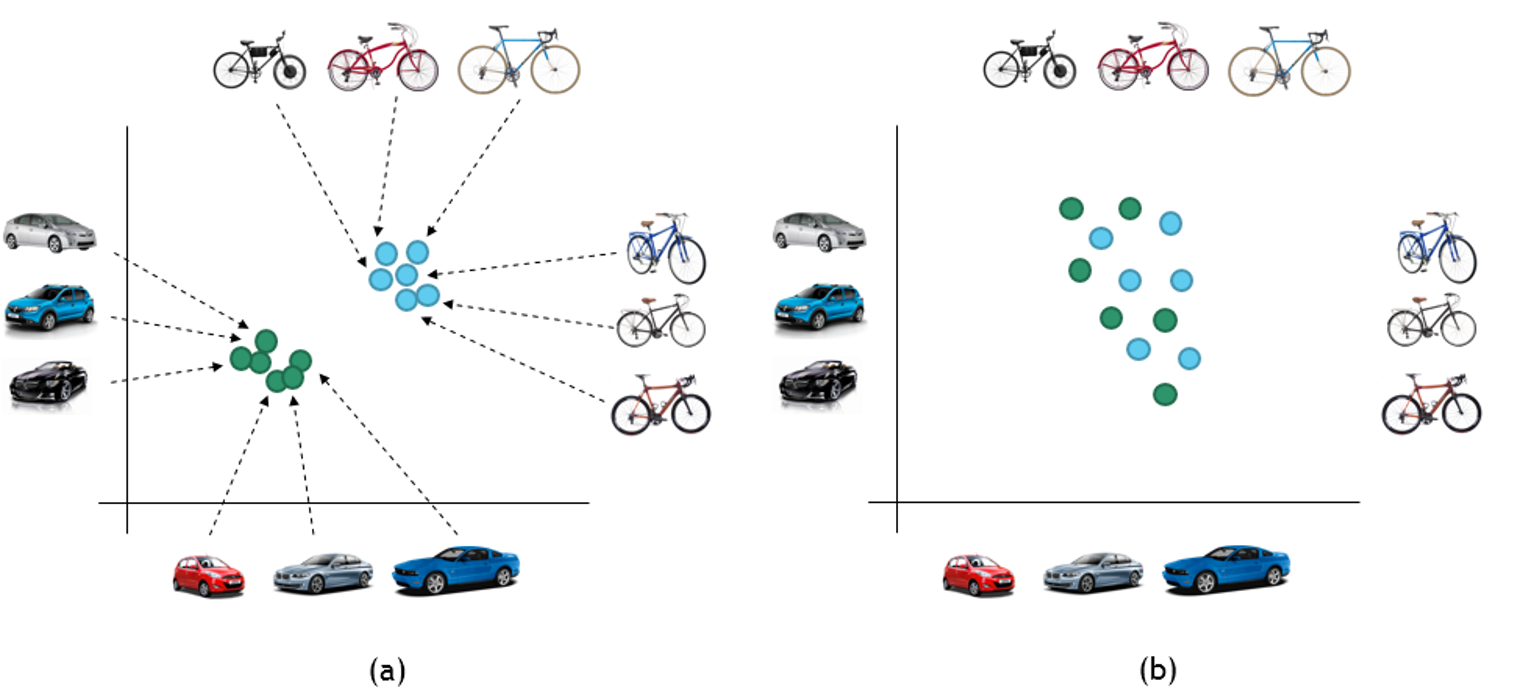
\includegraphics[scale=0.4]{image/ideal_feature.png}
\label{fig:feature}
\caption{Illustration of ideal and not-so-ideal features. (a) Ideal feature should have better separability from instance from different class and closely located with object form the same class. (b) Not-so-ideal features plot is jumbled all over the place and have low separability. This, however, can be compensated by using stronger classification algorithm.}
\end{figure}

% Handcrafted features
Many studies have proposed a wide array of feature extraction techniques. Until very recently, Scale-Invariant Feature Transform (SIFT) by Lowe \cite{lowe2004sift} and Histogram of Oriented Gradients (HOG) by Dalal and Triggs \cite{dalal2005hog} are the leading technique for feature extraction and produced decent performance on benchmark dataset. Both are similar in the sense that both first compute the gradient in the image and then count the gradient based on their direction into a histogram.

\begin{figure}[h]
\centering
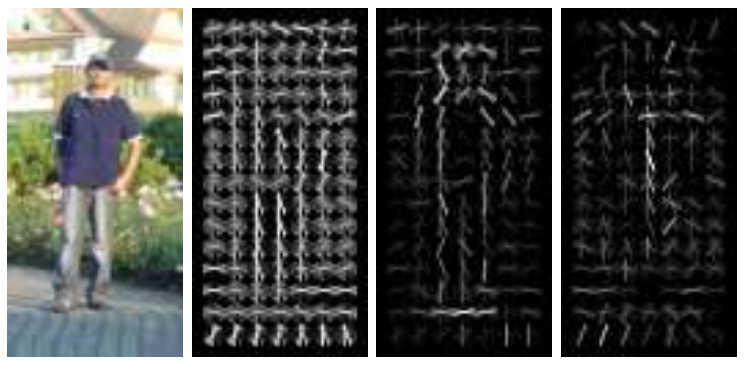
\includegraphics[scale=0.4]{image/hog.png}
\label{fig:hog}
\caption{Illustration of HOG features applied on image of a person.}
\end{figure}

Some study extends these features into mid-level representation by clustering nearby features (using k-means clustering for example). The number of features that fall into a specific cluster is then aggregated into some bag of visual word. However, this kind of hand-crafted features still cannot reach the level of human performance.

The trend shifts, there comes the initiative to learn the features directly from data. This is partly motivated due to the abundance of image data, mostly coming from the internet. There are two different approaches for this, the unsupervised learning and supervised learning.

Unsupervised feature learning works with image without label. It tries to learn generic features of object, regardless of their class. It is more advantageous because most of the data comes unlabeled and the extra effort to annotate the image with labels can be expensive and time-consuming.

One technique that implement this idea is Sparse Autoencoder. In its simplest form, it is a variant of neural network with the number of hidden neuron fewer than the dimension of the input. It then forces the network to learn compressed, low-dimensional representation of the image. Figure \ref{fig:autoencoder} illustrates some example features learned from this network.

\begin{figure}[h]
\centering
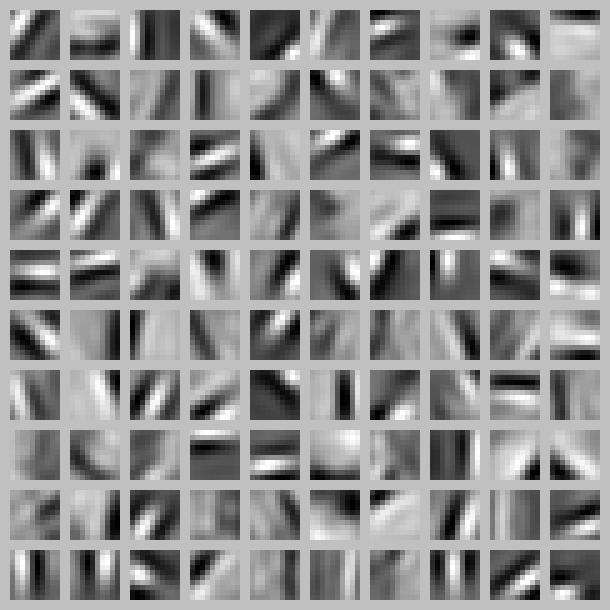
\includegraphics[scale=0.3]{image/autoencoder.png}
\label{fig:autoencoder}
\caption{The features learned from MNIST dataset. Each image correspond to edge at different location and orientation.}
\end{figure}

Supervised feature learning works with labeled image. One technique that successfully implement this idea is Convolutional Neural Network (ConvNet). It is originally proposed by LeCunn et al. \cite{lecunn1999} for handwriting document classification. This method is starting to gain momentum with the success of the seminal work of Krizhevsky et al. \cite{krizhevsky2012cnn} that produce stellar performance, by beating previous state-of-the-art method by large margin, on the ImageNet large scale recognition problem \cite{imagenet}. 

Part of this success can also be attributed to the abundance of labelled training data. ImageNet contains 1.2 million labelled training images from 1000 different categories. Another factor is the advance in Graphical Processing Unit (GPU) which makes training large amount of data feasible. Combining these factors with the learning capacity of a ConvNet makes the result possible.

\begin{figure}[h]
\centering
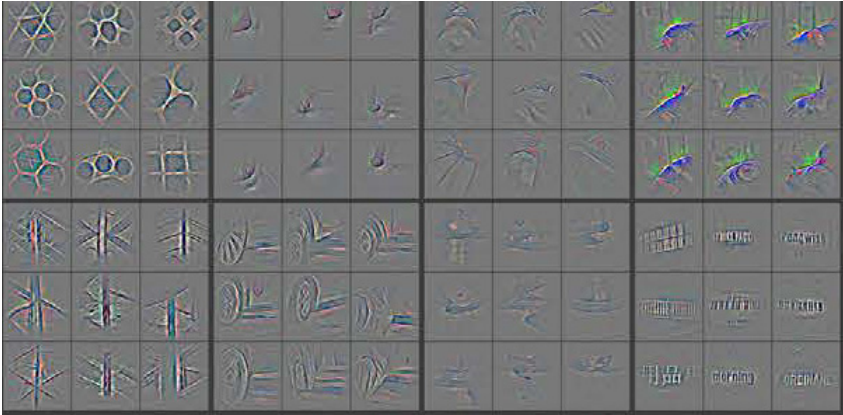
\includegraphics[scale=0.3]{image/cnn.png}
\label{fig:cnn}
\caption{Visualization of features learned from ConvNet.}
\end{figure}
[Visualization of features learned from ConvNet that generalize well to other dataset]

Figure \ref{fig:cnn} shows the example of features learned from a ConvNet, taken from Zeiler and Fergus \cite{zeiler2014} paper. Further research has showed that the feature produced from this network to be highly discriminative, even across different tasks and datasets. Study by Razavian et al. \cite{razavian2014} shows that the features coming from the last second fully-connected of ConvNet trained on ImageNet with simple linear classifier such as Support Vector Machine (SVM) produced top and near state-of-the-art performance in many typical vision tasks such as object classification, fine-grained recognition, and image retrieval. 

The result is pushed even further by finetuning the network with the target dataset. Finetuning works by taking the previously trained network, for example, the AlexNet, and retrain it with target dataset. This works particularly well, rather than training the network from beginning, especially if the target dataset has limited number of training data. This kind of learning, transfer learning, has been reported to produce better result on many occasions \cite{azizpour2014}.

One of the latest example that utilize this power of finetuning is the algorithm Region with CNN (RCNN). RCNN is a object detection algorithm that combines the highly discriminative features with a better search strategy. RCNN employs region proposal algorithm, selective search, that return ~2000 regions that is very likely to contain object. These two makes RCNN to get state-of-the-art result on benchmark dataset and made impressive improvement over previous methods.

This thesis work tries to extends the usability of RCNN. The standard RCNN needs the exact bounding box annotation for each object in the image for finetuning. However, this kind of annotation is more expensive than simply labeling the whole image. Therefore, we tries to bypass this needs and figure out a way to finetune with only whole image label. This kind of learning between the fully supervised and unsupervised is dubbed as weakly supervised learning.

The proposed general setup is as follows. First, we use a region proposal algorithm that can give confidence score that shows how likely a region to contain object. There are several possible candidates such as objectness \cite{obj} and EdgeBoxes. Hosang et al. \cite{hosang2014} provide extensive review of popular algorithm and then outline their strength and flaws. We pick top k regions and then extract them into individual image and and give the label from their source, whole image label.

These regions are then used for finetuning ConvNet that has previously been trained using ImageNet 1.2 million training images in 300,000 more iterations. This finetuned network will then be fed to the standard RCNN pipeline. The performance will be assessed using PASCAL 2007 detection dataset. It will be compared to the non-finetuned network, finetuned network with object bounding box annotation, and network finetuned with whole image.


\chapter{Literature Review}
\section{Convolutional Network (ConvNet)}
In this section, the development of neural network leading up to ConvNets is briefly summarized.

\subsection{Artificial Neural Network}
% Single neuron
The first neuron model is proposed by McCulloch and Pitts \cite{mcculloch1943neuron}. This model is a highly simplified version of neuron cell in brain. It works by multiplying the input vector with the neuron's weight vector. This value is then fed into an activation function. One activation function that can be used is a step function which acts as some kind of threshold operation. If this value exceeds certain $\theta$, then this neuron is firing. In other words $ a = \sum x_i w_i $ and:
\begin{equation}
y = 
	\begin{cases}
	1 & \text{if } a \geq \theta \\
	0 & \text{otherwise}
	\end{cases}
\end{equation}

This type of neuron is also called Threshold Logic Unit (TLU). Figure \ref{fig:neuron} illustrates the concept of this type of neuron.

\begin{figure}[h]
\centering
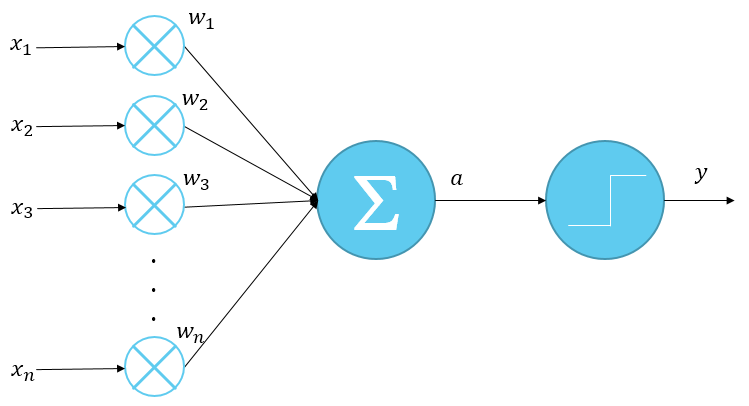
\includegraphics[scale=0.3]{image/neuron.png}
\label{fig:neuron}
\caption{Standard model of a neuron.}
\end{figure}

To update the the weight of the network to learn from the data, there are two update rules that is usually used, the perceptron rule and the delta rule. Perceptron rule was originally perceived by Rosenblatt \cite{rosenblatt1957perceptron} where to update the neuron we can just simply add the input vector to the weight vector if the output is misclassified. In other words: 
\begin{equation}
\begin{split}
\Delta w & = \alpha (t-y) \bm{x} \\
w(t+1) & = w(t) + \Delta w
\end{split}
\end{equation}
where $\bm{x}$ is the input vector, $alpha$ is the learning rate, $t$ is the target output, and $y$ is the output of the network.

There is a convergence theorem that states that if the data is linearly separable, then the perceptron learning rule will eventually converge, no matter the learning rate. However, perceptron suffer from the early stopping where if there were no training error, the network stopped learning even though the resulted network still has large validation error.

Delta rule, also known as Widrow-Hoff rule, works by minimizing a loss function. This loss function is defined as the sum of the difference between the target label and the output of the network with linear activation function. The delta rule empirically generalize better than perceptron. The update rule is defined as:
\begin{equation}
\begin{split}
\Delta w & = \alpha (t-y) g'(a) \bm{x} \\
w(t+1) & = w(t) + \Delta w
\end{split}
\end{equation}
where $a$ is the dot product between input vector and weight vector and $g'$ is the derivative of the activation function used. It is pretty similar with perceptron, with the exception of different activation function.

However, this type of networks has limitation that it can produce linear classifier. Even some kind of simple non-linear problem such as XOR problem cannot be solved. One way to alleviate this problem is by stacking one layer of neural network on top of other to build a multi-layer neural network. The input for the next layer is simply the output from the previous layer. The layer in the middle between input and output vector is usually called hidden layer. It has been shown that this kind of network with one hidden layer can be used to approximate any continuous function given sufficient hidden neuron \cite{cybenko1989}. Figure \ref{fig:multilayer} shows one instance of a multi-layer neural network.

\begin{figure}[h]
\centering
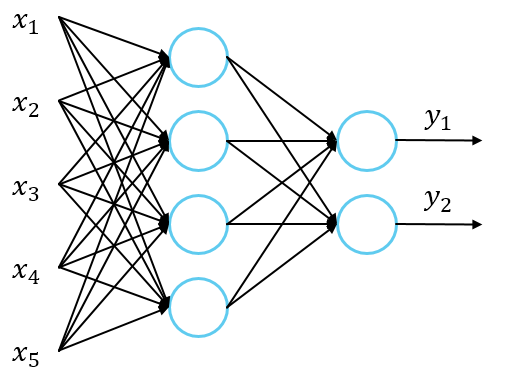
\includegraphics[scale=0.4]{image/multilayer.png}
\label{fig:multilayer}
\caption{One example of a multi-layer neural network. In this case, the input have 5 dimensions, there are 4 hidden neuron, and 2 target classes.}
\end{figure}

The caveat is then how to update the weight of the network, because we only know the error from the last layer. The found solution is by using threshold-like function, such as sigmoid function, and then performing chain rule to derive the update formula for each weight in different layers. This update formula is called Backpropogation \cite{rumelhart1986backprop}. Two popular choice for sigmoid function is $\frac{1-e^{-x}}{1+e^{-x}}$ or $arctan(x)$. Figure \ref{fig:sigmoid} shows the plot of a sigmoid function.

\begin{figure}[h]
\centering
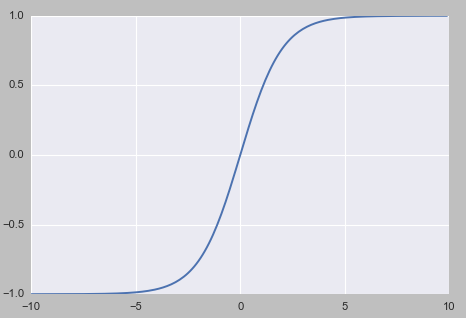
\includegraphics[scale=0.5]{image/sigmoid.png}
\label{fig:sigmoid}
\caption{Sigmoid function.}
\end{figure}

\subsection{ConvNet}
A Convolutional Neural Network (ConvNet) is a variant of the multi-layer neural network. It is inspired by the visual cortex in retina, where there are small sub-region in the cell that are highly sensitive, called receptive field. It is first proposed by Lecun et al. for document handwriting recognition \cite{lecun}.

There are two different paradigms that implement this receptive field concept. The first is sparse connectivity. A neuron in this network do not need to be connected to all the neurons from the previous layer. For example, a neuron in layer $i$ only need to be connected to limited number of spatially adjacent neuron on layer $i-1$. Figure \ref{fig:sparse} illustrates this concept.

\begin{figure}[h]
\centering
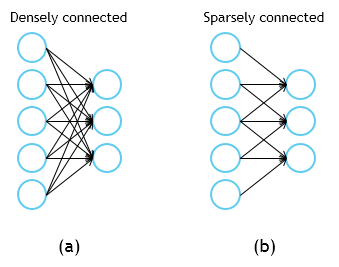
\includegraphics[scale=0.5]{image/sparse.png}
\label{fig:sparse}
\caption{Illustration between different connection. (a) Densely connected network connect all neuron from previous layer to the current one. (b) Sparsely connected network only connect limited number of neuron. In this case it is 3 spatially adjacent neurons.}
\end{figure}

The second paradigm is shared weight. It means that the weight are the same for all neurons on the same layer, usually called as feature map. This will ensure that the distinct features will be detected regardless of their position in the input. Figure \ref{fig:shared} illustrate the concept.

\begin{figure}
\centering
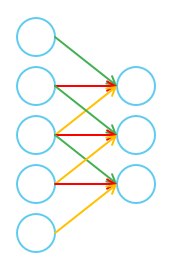
\includegraphics[scale=0.5]{image/shared.png}
\label{fig:shared}
\caption{Shared weight. Weight connection with the same color have the same value.}
\end{figure}

This two concepts together ultimately is just a convolution operation of an image with a kernel. Therefore, in ConvNet we are trying to learn the most discriminative kernel that can distinguish different objects instead of designing it by hand. It also has the advantage of having fewer parameter to train than a fully connected one.
This become the basis of the work of Krizhevsky et al. that change the landscape of computer vision.

\begin{figure}
\centering
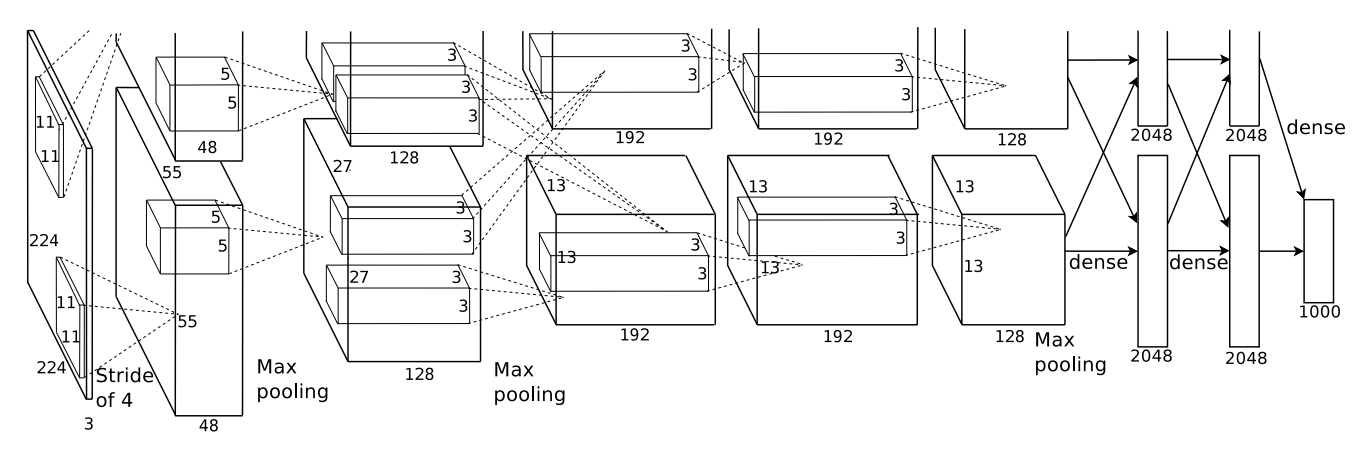
\includegraphics[scale=0.35]{image/alexnet.png}
\label{fig:alexnet}
\caption{The architecture of alexnet.}
\end{figure}

Figure \label{fig:alexnet} shows the architecture of said network. This network is composed of 5 convolutional layers, each followed by a max-pooling layer and Rectified Linear Unit (ReLU), followed by 2 fully-connected layers and lastly softmax layer to generate prediction. This network used three additional to boost the performance.

First is max-pooling. Max-pooling partitions the image into non-overlapping rectangular region, and for each region, outputs the maximum value. It has the advantage of reducing the computation cost and also provide some form of translation invariance into the network.

Second, Rectified Linear Unit (ReLU) as the activation function. $max(a, 0)$. This solves the problem of vanishing gradients that often happen when training a deep, multi-layer neural network with backpropagation. As the gradient goes deeper from the output layer to the hidden layer, the gradient value quickly diminish to zero which makes the network slow to learn.

\begin{figure}
\centering
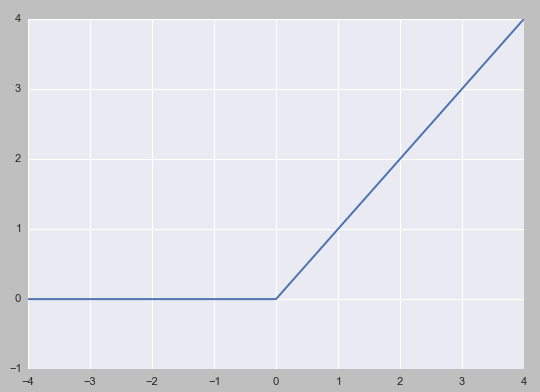
\includegraphics[scale=0.5]{image/relu.png}
\label{fig:relu}
\caption{Rectified Linear Unit. It is simply a linear activation function where value below zero is discarded and return as 0.}
\end{figure}

Third, Dropout as regularization method to prevent overfitting. This is done by setting the output of the neuron to 0 with 50\% probability. As a result it prevents neuron co-habitation and forces each neuron to independently learn the robust features.

This model is trained using GPU for 2 weeks with 1.2 million training data and achieved state-of-the-art performance on ImageNet Large Scale Visual Recognition Competition (ILSVRC) \cite{alexnet} with a large margin, over 10\% different than the previous winner.

[features learned from ConvNet, layer by layer]

\subsection{ConvNet as Black-box feature descriptor+Finetuning}
ConvNet works great for ImageNet. However, to train this large network with hideous number of parameter, a large number of training data and computation time and power is also required. This what is hinder.

However, surprisingly, it has been discovered. Now we can just take, and then train a linear SVM on top of this extracted features.
Study by Razavian et al. \cite{razavian}

Finetuning is performed by taking the previously trained network, and then replacing the last layer. Usually the learning rate is reduced for every other weights except that last replaced layer.

\section{Object Proposal}
% Traditional approach
There is a big shift in object detection world. Previously, a densely sampled sliding window is taken at all possible position and scale. It worked well, for example in the case of face detection \cite{violajones}. But when we start to take into account general object detection with different aspect ratio, the search space is simply become too big to fully explore. A standard image can produce up to million of windows to be evaluated. This can become prohibitively too slow to process.

[image of sliding windows]

% object proposal
Recent approach prefer to generate 1000-2000 candidate windows with high likelihood to contain object. The criteria to generate this boxes vary between algorithm, for example, by exploiting segmentation. It has the advantage of significantly speeding up the detection process. It can also produce better result by reducing the number of false positive rate.

[Example of object proposal. Notice, how is located near the object in the image]

% Explain objectness
Some notable algorithms are briefly described here.
Objectness \cite{alexe2012objectness} tries to create generic object measure to distinguish object windows from background ones. It use multiple cues such as multi-scale saliency, color contrast, edge density. It also introduces a new criterion based on the location and size of the window int he image itself, ignoring the pixels value inside the windows. It can generates up to 2000 windows in 4 seconds, in average.

% Explain selective search
Selective Search \cite{selectivesearch} performs hierarchical grouping from oversegmented region produced from Felzenszwalb and Huttenlocher graph segmentation algorithm \cite{felzenszwalb}. The grouping is done based on multiple criterion, such as color similarity, texture similarity, size (small regions should be fused with another small regions first), and fill to close gaps between regions. Higher number of proposal is obtained from combining the result from different parameters of such grouping.

[selective search steps]

% Explain Binarized Normed Gradient (BING)
BING \cite{bing} tries to distinguish object windows by looking at the norm of the gradient of the image window after it has been resized to small fixed size (e.g. 8x8). The approximated, binarized version of this which utilize binary operation such as ADD and BITWISE SHIFT, is very fast. It can achieved up to 300 frame per second on a single laptop CPU.

% Explain EdgeBoxes
EdgeBoxes \cite{zitnick2014edgeboxes} try to generate object bounding box proposals directly from edges. It used the observation that the number of contours fully enclosed by a bounding box shows how likely it is to contain object. It also used smart data structure to quickly generate the bounding box.

[edgeboxes]

% Penutup
Some algorithms provided ranking as some sort of confidence whether the region contains object or not. For a complete treatment of popular object proposal algorithm, refer the work of Hosang et al. \cite{hosang}.

\section{Region with CNN (RCNN)}

Object detection is a harder problem than object classification. Unlike classification, detection requires the location of the object inside the image. The second challenge is the number of labeled training data is scarce. The current amount of training data is insufficient to train a large ConvNet from scratch in order to get good feature representation.

Region with CNN features (RCNN) is the latest object detection algorithm that producing state-of-the-art result on many benchmark dataset such as PASCAL 2007 detection set and ImageNet detection problem. RCNN first solve the localization problem by using bottom up region proposal to get candidate object bounding boxes. For the second problem, RCNN use pre-trained ConvNet on large dataset (ILSRVC) followed by domain-specific fine-tuning on target dataset (PASCAL).

The general framework of RCNN is as follows. First, RCNN use class-independent region proposal algorithm such as Selective Search to generate around 2,000 proposals for each image. Then each region is warped to a fixed size to match the size of the input of the ConvNet. The features from the last fully-connected layer are then extracted. This features is then classified using pre-trained SVM classifier. Figure \ref{rcnn} shows the diagram of the RCNN system. Some detection results is showed in Figure \ref{rcnn_detect}.

[figure rcnn system]

[some detection result of RCNN]

\section{Weakly Supervised Object Detection}
Object detection usually needs the object bounding boxes annotation to train the detector. However, this kind of data is rarely available and it is more expensive to obtain compare to whole image label. Therefore, it is beneficial if we can train a detector without this additional annotation. Techniques that implement this kind of data is termed weakly supervised object detection.

Here we give brief review on some of the most common and notable algorithms in this field. Work by Wang et al. \cite{wang2014lcl}, called Latent Category Learning (LCL), try to learn hidden subcategory for each region using probabilistic Latent Semantic Analysis. He then also uses ConvNet as feature representation and SVM for classification.
Cinbis et al. \cite{cinbis2014mil} treat this problem as multiple instance learning and use multi-fold approach where the data is divided into train and validation part. The SVM is trained on training data and then it is used to refine the localization of the validation part. This process is performed iteratively for every fold.

\chapter{Experiment and Result}
\section{Dataset}
The dataset used is PASCAL Visual Object Class 2007. This dataset contains nearly 10000 images of 20 different visual classes.

The measurement used is average precision. This is a more accurate assessment than simply accuracy.

\section{Program}
We are using Caffe.
Caffe is designed so an experiment parameter can be changed by changing the parameter prototxt file.
There is a pre-trained model which mimic, with slightly different. It is reported 2\% accuracy different. This network will then be referred throughout the rest of this thesis as caffenet.

Caffe also provide a model zoo, where researcher all around the world can provide a model they are trained with different architecture. It will be interesting to compare with latest network.

As for the RCNN code itself, the author provide it online in a github repository: .

\section{Experiment}

The first result is using the pre-trained caffenet. This result will act as lower bound for the rest of the experiment.

The second experiment is by running RCNN with finetuned network with bounding box annotation. This will act as upper bound.

There is a solid improvement of 8\% from previous experiment. This solidify the hypothesis that finetuning to the target dataset really works.

We then finetune the network with. The strategy is as defined in the paper. Every region with 0.5 is considered as positive samples and.

Because the number of samples can easily reach million of datapoints, negative hard mining is performed.

We tried to build several models. The first, most simple approach is to finetune the network with whole image. In PASCAL, one image can contains many object from different classes.

The second model, we try to include image with multiple. As caffe in the time of this writing have not support multi label, we list multiple times as different data.

If we try to include more training image, it is fear that it will corrupt the network with noise.

This might turned out to be.

\section{Discussion}
As can be seen on the. Judging from the plot of loss and accuracy during finetuning, it seems like the network is not learning at all.
This can probably be attributed to the low number of training images.

Another part that has not been done is the weakly supervised learning in SVM side. The SVM training still needs the full bounding box annotations to train.

\bibliographystyle{plain}
\bibliography{ref.bib}

\appendix
\addappheadtotoc
\chapter{RDF}\label{appA}

\begin{figure}[ht]
\begin{center}
And here is a figure
\caption{\small{Several statements describing the same resource.}}\label{RDF_4}
\end{center}
\end{figure}

that we refer to here: \ref{RDF_4}
\end{document}
